The primary goal of Makahiki is to support energy competitions. \autoref{related:competitions} will look at the current state of energy competitions in the United States and how we can improve upon them. \autoref{related:serious-games} will look at the growing field of \emph{serious games} and how we can use game design techniques to engage players while increasing their energy awareness. Finally, \autoref{related:evaluations} will look at usability evaluations and how we can collect metrics in order to assess the usability of our system.

\section{Energy Competitions}
\label{related:competitions}

Ever since Harvard hosted the first Green Cup in 1990~\cite{harvard-greencup}, universities all over the nation have started holding dorm energy competitions. \autoref{competitions-duke} will look into Duke University's Eco-Olympics.  \autoref{competitions-oberlin} will look into Oberlin College's Ecolympics, which is the first energy competition based on Lucid Design Group's Energy Dashboard. Finally, \autoref{competitions-evaluation} will do a brief comparison and evaluation of a few other dorm energy competitions and how they compare to each other.

\subsection{Duke University's Eco-Olympics}
\label{competitions-duke}

Duke held their first Eco-Olympics~\cite{duke-eco-olympics} in 2002.  The Eco-Olympics not only involves energy conservation, but water conservation and waste reduction as well.  However, energy reduction plays a significant part in the competition as it is one of the largest components of the Eco-Olympics in terms of possible points.  Each week, the organizers get meter readings from the dorms and compare the readings with the dorm's respective baseline reading in order to calculate a per-capita reading.  This baseline reading is obtained in September, so it reflects usage when students are living in the dorm.   The key thing to note is that dorms are not directly competing against each other, as dorms vary in size and have differing energy requirements.  Also, the weekly readings are to provide feedback on how residents of each dorm are doing.  Points are only awarded at the end of the competition and the dorm with the lowest per-capita reading receives the full number of points.

\begin{figure}
	\centering
	\includegraphics[scale=0.25]{images/duke-ecolympics.eps}
	\caption{Duke Eco-Olympics}
\end{figure}

The other major component of the Eco-Olympics is participation in events.  Dorms are awarded points based on the percent of residents who attend each event.  The number of points for each event may vary, but the total points is comparable to the possible number of points for energy conservation.  These events can also involve conservation-related games.  The individuals participating in these games can also win prizes, providing additional incentive for dorm residents to participate.

The web page for the Duke Eco-Olympics is very basic.  The interface is similar to most content management systems in that there is a row of tabs at the top and the content listed below.  However, there is no place for user generated content, very little energy conservation related content, and, outside of a Google calendar, very little ``Web 2.0'' design to it.  The lack of these three things give users little reason to visit the page other than to see the weekly current standings and upcoming events.

\subsection{Oberlin College's Ecolympics}
\label{competitions-oberlin}

Oberlin College in Ohio also runs dorm energy competitions.  Instead of going with manual meter readings, Oberlin has partnered with Lucid Design Group to create their Campus Resource Monitoring System~\cite{oberlin-comp}.  The Campus Resource Monitoring System is active year-round and retrieves real time electricity and water usage from 26 buildings~\cite{lucid-oberlin} on campus.  The system provides graphs and statistics and are presented to users in a clean and interactive way.

The first competition that used the Campus Resource Monitoring System proved to be a success.  A study conducted during the 2005 dorm energy competition found that dorms with real time feedback reduced their energy consumption by 55 percent while dorms with ``medium resolution" feedback only reduced their energy usage by 32 percent~\cite{oberlin-goals}.  In total, the competition saved 68,000 kWh which translated to a savings of \textdollar5,100.

\begin{figure}
	\centering
	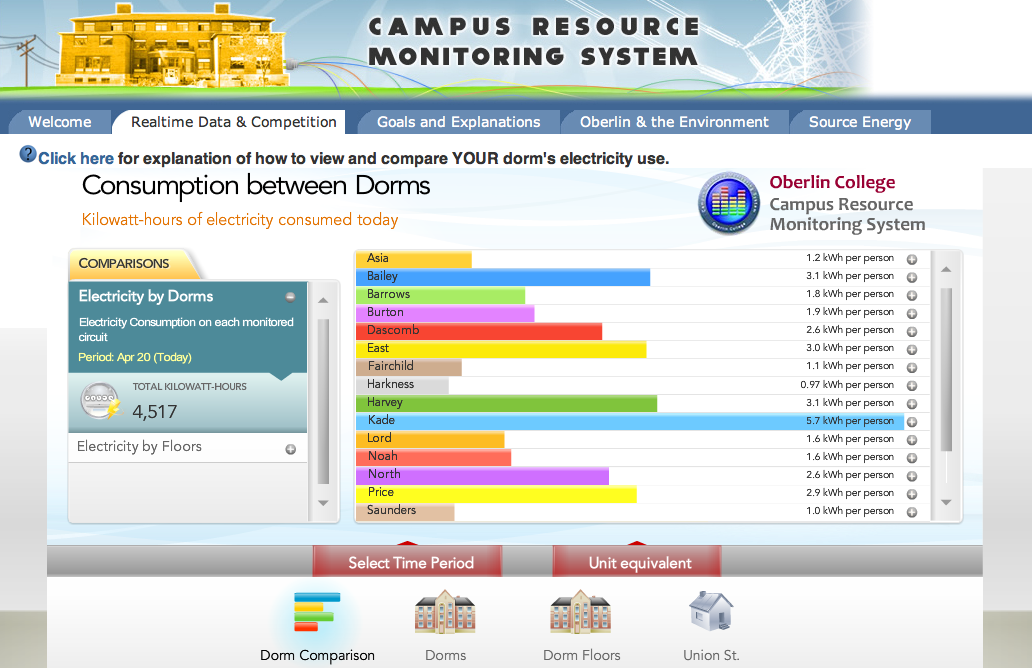
\includegraphics[scale=0.25]{images/oberlin-crms.eps}
	\caption{Oberlin College Campus Resource Monitoring System}
\end{figure}

While Oberlin held yearly dorm energy competitions for some time, they had their first sustainability competition, called the Ecolympics, in March of 2008~\cite{oberlin-history}.  The Ecolympics at Oberlin are run at about the same time as the dorm energy competition, but the two competitions are separate.  Dorms earn points for participation in events like attending environmentally themed lectures and film screenings~\cite{oberlin-news}.  Depending on the event, participants can also win individual prizes.  However, participation in these events are tracked separately from the campus resource monitoring system.

\subsection{Competition Evaluation}
\label{competitions-evaluation}

Dorm Energy competitions are becoming increasingly prevalent across the United States. Chelsea Hodge found that 163 universities and colleges held or planned to hold an energy competition during the 2010-2011 academic year~\cite{hodge-competitions}. Furthermore, 40\% of these organizations are holding a competition for the first time. Hodge also found that these competitions are successful, with the top 25\% of universities reducing energy usage within a building by 12\% on average.

\autoref{feature-matrix} outlines a few college and university energy competitions and the features they have.

\begin{table}[t!]
	\begin{tabular}{| p{5cm} || p{2cm} | p{2cm} | p{2cm} | p{2cm} |}
		\hline
		Organization & Energy Input & Participation Competition & Mobile Viewable & Facebook page \\
		\hline
		Duke University & Manual & Yes & Yes & No \\
		Oberlin College & Real-Time & Yes & No & Yes\\
		Brandeis University~\cite{brandeis} & Manual & No & Yes & No\\
		Bowdoin College~\cite{bowdoin} & Real-Time & No & No & No\\
		Harvard University & Manual & Yes & Yes & No\\
		Indiana University~\cite{indiana-energychallenge} & Manual & No & Partial & Yes\\
		Northeastern University~\cite{northeastern} & Manual & No & Yes & No\\
		Northwestern University~\cite{northwestern} & Manual & No & Yes & Yes \\
		Ohio University~\cite{ohio-reschallenge} & Manual & No & Yes & Yes\\
		Rice University~\cite{rice-sustainability} & Manual & No & Yes & No\\
		Stanford University~\cite{stanford-energybowl} & Manual & No & Yes & No \\
		Tufts University~\cite{tufts-competition} & Manual & No & Yes & No \\
		University of North Carolina - Asheville~\cite{unc-asheville} & Manual & No & Yes & No \\
		University of North Carolina - Chapel Hill~\cite{unc-chapelhill} & Manual & Yes & Yes & Yes \\
		University of Iowa~\cite{iowa-sturrier} & Manual & Yes & Yes & No \\
		University of Rhode Island~\cite{greenuri} & Manual & No & Yes & No \\
		University of Virginia~\cite{virginia} & Manual & No & Yes & No \\
		Wellesley College~\cite{wellesley} & Manual & No & Yes & No \\
		Wesleyan University~\cite{wesleyan} & Manual & No & Yes & No \\
		Yale University~\cite{yale-greencup} & Manual & No & Yes & No \\
		Williams College~\cite{williams} & Manual & No & Yes & No \\
		Western Washington University~\cite{wwu-goforthegreen} & Manual & No & Yes & No \\
		\hline
	\end{tabular}
	\caption{University dorm energy competition implementations}
	\label{feature-matrix}
\end{table}

Duke University and Oberlin College both hold dorm energy competitions, but the way these two colleges implemented the competition are very different.  While Lucid Design Group's building dashboard is very clean and interactive, some competition organizers use a static site like Duke's.  This is understandable, since using hardware and software provided by Lucid Design Group is relatively expensive.  Thus, organizers that want to run an energy competition with little to no funds are relegated to manually reading the meter and updating the standings and web site accordingly.  The web interface of these competitions is fairly sparse, with a simple, static layout of tabs and content.

Also, the goal of most university sustainability organizations is to improve energy awareness.  To accomplish this, many organizations have competitions where dorms earn points by participating in energy awareness events.  Usually, these competitions are held as another component of an overall competition. In Harvard's Green Cup~\cite{harvard-greencup}, energy reduction is a mere 10 percent of the overall competition. The other 90 percent includes recycling and waste reduction, participation in the Harvard Sustainability Pledge, and developing ecological projects.

However, the implementations of these dorm energy competitions have not kept up with the advances of technology and the web.  First, none of the dorm energy competitions surveyed seem to have a mobile device (iPhone, iPad, Android) interface.  Simple energy competition websites like Duke's, Stanford's, and Yale's load the full version of their web site on the iPhone.  Because mobile devices have small screens, this means that a user would have to zoom in to read the content and click on links.  Furthermore, because the iPhone and iPad do not support Adobe Flash at this time, competition websites that use Flash may not load.  In a few pages, like Indiana University's Energy Challenge, most of the page still loads.  However, pages that use Flash extensively do not load on these devices at all.  \autoref{iphone-comparison} shows screen shots of Oberlin College's Campus Resource Monitoring System, Indiana University's Energy Challenge,  and Duke's Eco-Olympics as seen on an iPhone.

\begin{figure}
	\centering
	\subfigure[Oberlin College]
	{
		\label{oberlin-iphone}
		\includegraphics[width=4cm]{images/oberlin-iphone.eps}
	}
	\hspace{1cm}
	\subfigure[Indiana University]
	{
		\label{indiana-iphone}
		\includegraphics[width=4cm]{images/indiana-iphone.eps}
	}
	\hspace{1cm}
	\subfigure[Duke University]
	{
		\label{duke-iphone}
		\includegraphics[width=4cm]{images/duke-iphone.eps}
	}
	\caption{Dorm energy web sites as they appear on an iPhone.}
	\label{iphone-comparison}
\end{figure}

Another advancement in technology that these competitions do not involve is the use of social networks like Facebook.  Since most college students already have an account on one or many social networks, having a presence there provides opportunities for them to share their activities.  To spread the word of their dorm energy competition, Virginia Tech has a page on Facebook for their 2010 Eco Olympics~\cite{vt-facebook}.  Duke University also has yearly Facebook group pages for their Eco-Olympics~\cite{duke-facebook}.  However, Facebook users like to share what they are doing and what they find interesting, and this cannot be accomplished with pages and groups alone.

Despite these shortcomings, Lucid Design Group's Building Dashboard has become a very popular option. Lucid's latest project is the Campus Conservation Nationals~\cite{lucid-ccn}, a sustainability competition involving multiple colleges and universities across the United States and Canada. Their pilot competition had over 40 participants and was held in November 2010. They succeeded in reducing energy usage by 508,000 kilowatt-hours and water usage by 730,000 gallons. Their next competition will be in 2012, where they have over 170 colleges and universities signed up.

\section{Serious Games}
\label{related:serious-games}

Michael Zyda defines serious games by building up the definition from games and video games~\cite{zyda-from-visual-sim}.  Zyda defines a serious game as ``a mental contest, played with a computer in accordance with specific rules that uses entertainment to further government or corporate training, education, health, public policy, and strategic communication objectives.''  While integrating games with real-world tasks is not a novel idea, advances in technology allowed Zyda and serious game makers to look at simulations of real-world activity.  The key turning point was the development of the game ``America's Army'', a third-person military shooting game developed initially as a recruiting tool for the U.S. Army.  While there was initial skepticism that the game would improve real-world skills, they found that soldiers who played the game generally performed well in real-world tests.

Not all serious games need to involve virtual simulations of the environment.  EVOKE (http://www.urgentevoke.com) is a serious game developed by the World Bank Institute and is a game where people learn to find ways to change the real world.  Instead of having players control a virtual avatar in a simulated world, players log in to the EVOKE website where they are given a set of quests and missions.  Quests take place on the EVOKE website and involve the player answering questions in order to create a story.  Missions are things that players do in the real world.  These missions require ``evidence'' (either a blog post, a video, or a photo), which need to be submitted and approved in order to get credit.

Jane McGonigal, the creator of EVOKE, is no stranger to the idea of using games for more than just entertainment.  In her book ``Reality is Broken'', she states that gamers seek escape in games because reality needs fixing~\cite{mcgonigal-reality-broken}.  She then describes these fixes to reality and bases them on techniques used in games to engage players and keep them interested.  While she starts with traditional computer and video games, she moves on to \emph{alternate reality games} games that involve people in the real world playing together.  Finally, she describes large scale alternate reality games that encourages players around the world to work together to figure out solutions to hypothetical global issues.  She describes a game called ``A World Without Oil'', where players are thrust into a hypothetical peak-oil situation where demand outstrips supply.  Players are then challenged to brainstorm ways to live their lives without dependence on oil and share their ideas with other players.  While player ideas are initially very simple, they get developed further as a result of feedback from other players in the game.

Serious games can engage people and help them become more productive and engaged. Byron Reeves observed that many adults are playing online games like World of Warcraft. These adults find themselves to be more engaged in their online quests than their real life jobs. If concepts from these online games can be incorporated in a compelling way toward real-life tasks, employees would be far more productive. In his book ``Total Engagement''~\cite{reeves-total}, Reeves studied how games transform the way people work and provides guidelines to creating games that increase real world productivity in the workplace. Components of games that can be applied to the workplace include:

\begin{itemize}
  \item Self-representation with avatars
  \item Three-dimensional virtual environments
  \item Narrative context
  \item Feedback
  \item Reputations, ranks, and levels
  \item Marketplaces and economies
  \item Rules that are explicit and enforced
  \item Teams
  \item Communication system that can be reconfigured by participants
  \item Time pressure
\end{itemize}

How do games motivate us and keep us engaged? McGonigal describes in her book a state called ``fiero'', which describes a feeling that people get when they feel their hard work has paid off. An example of this is when an athlete wins a gold medal or a sports team wins the championship. Typically, you will see people experiencing ``fiero'' with their hands in the air, with an expression of both happiness and relief. However, such a feeling is very difficult to attain in the real world. Games, especially ones that involve other players, can be designed to be competitive and rewarding. In that sense, McGonigal sees multiplayer games as being the ``ultimate happiness engine''.

The motivation and sense of accomplishment in games can be tied to learning. In researching the Navy's Damage Control Trainer, Curtiss Murphy examined the basic tenets that improve learning and compared them to the basic tenets of game design~\cite{murphy-science-learning}. He describes 6 laws of learning and ties each law directly to a game design technique. The links are summarized in \autoref{table:laws-game-design}

\begin{table}[t!]
	\begin{tabular}{| l | p{4cm} | p{7cm} |}
		\hline
		Law of Learning & Idea & Game Design Techniques \\
		\hline
		Motivation & Motivated students learn more & Flow: The fundamental attraction of games. Games are fun and require moment to moment choices. These lead to motivating experiences. \\
		Feedback & Feedback is how learners correlate actions with outcomes & Feedback loops in games help the learner correlate actions to outcomes. \\
		Practice & Practice is necessary for learning and mastery & Games use practice to encourage mastery.\\
		Positive Feelings & Learning is increased when associated with positive feelings & Games that are \emph{fun} create positive feelings and encourage the user to continue playing.\\
		Intensity & Intense experiences increase learning, interest, and retention & A person experiencing \emph{flow} is immersed and engaged with the activity.\\
		Choice/Involvement & Involvement and decision making can increase motivation, intensity, and positive feelings & Playing a game means making a series of interesting and meaningful decisions. Players are learning through their experience in the game.\\
	\hline
	\end{tabular}
	\caption{Laws of Learning linked to Game Design Techniques. Used with permission from Curtiss Murphy.}
	\label{table:laws-game-design}
\end{table}

\section{Usability Evaluations}
\label{related:evaluations}

Evaluating the usability of a website can be very costly.  They can involve specialized tools such as eye-tracking devices and include many users.  In 1994, Jakob Nielsen showed how organizations can cut the cost of these evaluations using what he calls ``discount usability engineering''~\cite{nielsen-guerrilla-hci}.  Discount usability engineering is based on three techniques; scenarios, simplified thinking aloud, and heuristic evaluation.  Scenarios involve very specific tasks and do not necessarily require full functionality.  Simplified thinking aloud reduces the number of subjects and involves taking notes rather than capturing video.  Finally, heuristic evaluation simplifies a list of rules to follow to ten ``rules of thumb''.

Steve Krug further builds upon these heuristics in his book ``Don't Make Me Think''~\cite{krug-dmmt}.  His main point is that new users do not look at a website in the way you want them to.  In many cases, the designers of a website want users to read all of the provided content in order to make decisions.  However, Krug has found through eye tracking studies that users skim the content and try to find something that matches what they are looking for.  Krug also develops a usability test procedure based on Nielsen's techniques and walks through an example usability test with another user.

One important assumption in the example websites used in Krug's usability test walkthrough is that the user knows what they wish to accomplish in the website.  This is very different from our system, where it is likely that the user will not know what they can do within our website; only that it involves some kind of competition.  Krug's usability scenarios are based on basic tasks that users should be able to accomplish, so how can our subjects accomplish these scenarios if they do not know what they can do?

One approach is to provide time for the user to navigate around the site and figure out what they are able to do. In the book ``Interaction Design'', the authors describe a collaborative project between the Fred Hutchinson Cancer Research Center and Microsoft called ``Hutchworld''~\cite{preece-interaction-design}~\cite{cheng-hutchworld}.  Hutchworld is a three dimensional virtual world designed for patients within the cancer research center.  Within the virtual world, patients can access information about the center, interact with family members who are also logged in to Hutchworld, and participate in diversionary activities.  As part of developing the system, Microsoft conducted usability tests on Hutchworld.  Before getting to the usability test's scenarios, however, subjects were given five minutes to explore the virtual interface.  Subjects were given a chance to figure out how to move within the virtual interface and also find what content is available to them within Hutchworld.

How do we measure the usability of our system? Tullis and Albert provide various examples of usability metrics in their book ``Measuring the User Experience''~\cite{tullis-measuring-ux}. Since our usability procedure involves completing transactions, Tullis and Albert suggest measuring task success, user efficiency, issues-based metrics, self-reported metrics, and live website metrics. Task success is a fairly simple metric: given a task, does the user complete it or not? User efficiency is a measurement of the effort required for the user to complete the task. For example, we can measure this by the number of clicks or the amount of time spent to complete the task. Issues-based metrics involve measuring the number of times usability issues are encountered. These issues may manifest themselves as both verbal and non-verbal expressions of confusion or indecision. Self-reported metrics are based on user responses to questions. Finally, live website metrics involve the usage of the logs created by the website to evaluate the user.

% \section{Design}
% 
% Our initial goal in designing Makahiki was to create a energy competition that incorporated the latest advances in technology, including social networks and mobile devices. However, we also wanted to provide the energy literacy competition that a few other competitions have included. This pushed us to make sure the website was engaging and fun. Our users are not forced to use our system, so we must create a system that wants them to come back. Part of that is incorporating ideas serious games. However, we still need to show the system to users that match our target demographic. Not only does this make sure the system is usable, but we can also gain insight into how ``fun'' the game is.